\documentclass[tikz]{standalone}
\usepackage[utf8]{inputenc}
\usetikzlibrary{calc,perspective}

\definecolor{DarkBlue}{rgb}{0.0,0.0,0.6}
\definecolor{DarkRed}{rgb}{0.7,0.2,0.2}

\begin{document}

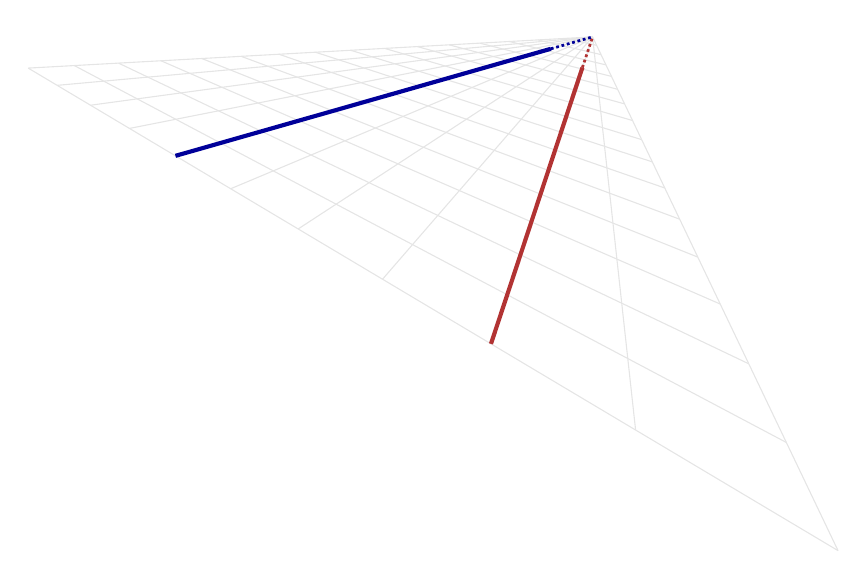
\begin{tikzpicture}[scale=3,3d view={-40}{30},perspective={p={(4,0,0)},q={(0,4,0)}}]

\foreach \y in {-2,-1.6,...,2}
\draw[gray!20] (tpp cs:x=0,y=\y,z=0) -- (tpp cs:x=4,y=0,z=0);

\foreach \x in {0,.25,...,4}
\draw[gray!20] (tpp cs:x=\x,y=.5*\x-2,z=0) -- (tpp cs:x=\x,y=-.5*\x+2,z=0);

\node (A) at (tpp cs:x=0,y=-1.2,z=0) {};
\node (B) at (tpp cs:x=0,y=.4,z=0) {};
\node (C) at (tpp cs:x=4,y=0,z=0) {};

\draw[line width=1.5pt,DarkRed] (A.center) -- ($(A)!.9!(C)$);
\draw[DarkRed,line width=1pt,densely dotted] ($(A)!.9!(C)$) -- (C.center);

\draw[line width=1.5pt,DarkBlue] (B.center) -- ($(B)!.9!(C)$);
\draw[DarkBlue,line width=1pt,densely dotted] ($(B)!.9!(C)$) -- (C.center);

\end{tikzpicture}

\end{document}